\chapter[Application of the SIS with Corrections method to the RIFA invasion]{Application of the SIS with Corrections method to the RIFA invasion}
\label{ch:ModelMethod}



{\color{red}
\section{Sequential Importance Sampling with corrections applied to the self-exciting point process} \label{sec:SISMethod}

In this section we apply a new Sequential Importance Sampling methodology to the model above in order to estimate position and time of founding of all observed and unobserved nests. As we have discussed in the introduction, during the eradication program locations of new nests are continuously acquired either through passive or active surveillance activities, while new nests are also continuously created. We will consider the locations and time of observation as correct information when we acquire it, however, only a limited number of colonies will be discovered at each observation while an unknown number of them will remain undetected. If an area is surveyed and deemed free of invaders this can be because there are no invaders to be detected or because we fail to make an observation. This can happen for example when nests are young and not easy to spot. At each step we will simulate plausible locations and founding times for all the undetected nests created in the past and for all the newly created nests. When receiving new data these simulations will need correction in order to get the most plausible configuration of nests in light of this data. We will therefore correct the simulation then adjust the weights in order to correctly represent our posterior.

\subsection{Bayesian inference in a partially observed state space} \label{subsec:POS}

In section \ref{section:simulationModel} we have defined the time intervals $\tau_j = (T_{j-1}, T_j]$ where $T_j$ is the time at which we receive a new set of observations. Then the interval of time $[T_0, T_i]$ from the beginning of the invasion $T_0=0$ to the time of the last detection $T_i$ will be partitioned in sub-intervals $\tau_j$ with $j = 1, \dots, i$.

Consider a system evolving continuously in time. The states of the system at times $T_j$ are represented by random sets $\vec{a}^{T_j} = (a^{T_j}_1, \dots, a^{T_j}_{N^{T_j}}) \in \mathbb{R}^{4\times N^{T_j}}$ where $N^{T_j}$ is the unknown number of nests alive at time $T_j$ and whose elements $a^{T_j}_k = (t_k^{T_j}, f_k^{T_j}, x_k^{T_j}, y_k^{T_j})$ with $k = 1, \dots , N^{T_j}$ represent the nests indexed by $k$ and containing 4 elements: the time of founding $f_k$, the time of observation $t_k$ corresponding to the time of deaths, and the coordinates $x_k$ and $y_k$.
The trajectory of the system from $T_0$ to $T_i$ is represented by the random set $\vec{A}^{T_i} = (\vec{a}^1, \dots, \vec{a}^{T_i})$. 

We are also going to define an \textit{observation set} $\vec{z}^{T_i} \in \mathbb{R}^{i \times M^{T_i} \times 3}$ where $M^{T_i}$ is the total number of nests detected up to time $T_i$. The vectors $z^{T_j}_l = (t^{T_j}_l, x^{T_j}_l, y^{T_j}_l)$ will contain the time of observation and coordinates of a nest. It will also be useful to define $\vec{Z}^{T_i} = (\vec{z}^1, \dots, \vec{z}^{T_i})$. Since our observations are exact, $\vec{Z}^{T_i}$ will fix the values of location and time of observation for $M^{T_i}$ nests $a^{T_m}_k$ leaving $N^{T_i}-M^{T_i}$ elements of $\vec{A}^{T_i}$ undetermined. We therefore define a function $\sigma_{T_i}: \mathbb{R}^{i\times N^{T_j}\times 3} \rightarrow \mathbb{R}^{i\times M^{T_j}\times 4}$ such that $\vec{Z}^{T_i} = \sigma_{T_i}(\vec{A}^{T_i})$.

Using a Bayesian approach, we can quantify information for all the nests that have not been observed by time $T_i$ using the model of the system and the data received.

At time $T_1$ our knowledge of the system is represented by a prior distribution with density $q(\vec{A}^{T_1})$ on $\Omega_{T_1} = \mathbb{R}^{N^{T_1}}$ and the posterior distribution after observing $\vec{Z}^{T_1}$ has density on $\Omega'_{T_1} = \sigma^{-1}(\vec{Z}^{T_1})$ given by:

\begin{equation*}
    p(\vec{A}^{T_1} | \vec{Z}^{T_1}) = \frac{q(\vec{A}^{T_1})}{r(\vec{z}^{T_1})}
\end{equation*}
where
\begin{equation*}
    r(\vec{z}^{T_1}) = \int_{\Omega'_{T_1}} q(\vec{A}^{T_1}) 
\end{equation*}
and the integral is over the elements of $\vec{A}^{T_1}$ that are not determined by $\vec{Z}^{T_1}$.

(NOTE: I need to define the metric here. I think it would be good to explain this exactly as Jon has done in his original notes on the method with the disintegration theorem. I guess this will perhaps depend on which journal we are going to submit the paper to).
Our knowledge of the trajectory of the system at time $T_j$ with $i \geq 2$, before we acquire the next observation matrix $\vec{z}^{T_i}$ is represented by a prior distribution with density $q(\vec{A}^{T_i} | \vec{Z}^{T_{i-1}})$ on the subspace $\Omega_{T_i} = \sigma_{T_i}^{-1} (\vec{Z}^{T_{i-1}}) \times \mathbb{R}^{4 \times N^{T_i}}$. After observing $\vec{z}^{T_i}$, many elements $\vec{A}^{T_i}$ with non zero prior density will be incompatible with the new observations, and the posterior density must therefore restrict $\vec{A}^{T_i}$ to $\Omega_{T_i}' = \sigma_{T_i}^{-1}(\vec{Z}^{T_i})$. The posterior density over $\Omega_{T_i}'$ will then be

\begin{equation*}
    p(\vec{A}^{T_i} | \vec{Z}^{T_i}) = \frac{q(\vec{A}^{T_i} | \vec{Z}^{T_{i-1}})}{r(\vec{z}^{T_i} | \vec{Z}^{T_{i-1}})}
\end{equation*}
were

\begin{equation*}
    r(\vec{z}^{T_i} | \vec{Z}^{T_{i-1}}) = \int_{\Omega'_{T_i}} q(\vec{A}^{T_i} | \vec{Z}^{T_{i-1}})
\end{equation*}

We will now use the model introduced in chapter \ref{section:model} for the RIFA invasion that defines the transition of the system from one state to the next. We firstly recall that this model is Markovian, therefore each $\vec{a}^{T_i}$ is conditionally independent of $\vec{A}^{T_{i-2}} = (\vec{a}^{T_1}, \dots, \vec{a}^{T_{i-2}})$, given $\vec{a}^{T_{i-1}}$. The transitional density distribution characterising the system will be the likelihood of the model in chapter \ref{section:model} which we will call $f(\vec{a}^{T_i} | \vec{a}^{T_{i-1}})$. It follows that at time $T_1$
\begin{equation*}
    q(\vec{A}^{T_1}) = f(\vec{a}^{T_1})
\end{equation*}
and for $T_i$ with $i \geq 2$:

\begin{equation*}
    q(\vec{A}^{T_i} | \vec{Z}^{T_{i-1}}) = f(\vec{a}^{T_i} | \vec{a}^{T_{i-1}}) p(\vec{A}^{T_{i-1}} | \vec{Z}^{T_{i-1}}) = \frac{f(\vec{a}^{T_1})}{r(\vec{z}^{T_1})} \prod_{j=2}^{i-1} \frac{f(\vec{a}^{T_j} | \vec{a}^{T_{j-1}})}{r(\vec{z}^{T_j} | \vec{Z}^{T_{j-1}})} \times f(\vec{a}^{T_i} | \vec{a}^{T_{i-1}})
\end{equation*}
on the space $\Omega_{T_i}$, so the joint posterior distribution will be

\begin{equation*}
    p(\vec{A}^{T_i} | \vec{Z}^{T_i}) = \frac{f(\vec{a}^{T_1})}{r(\vec{z}^{T_1})} \prod_{j=2}^{i} \frac{f(\vec{a}^{T_j} | \vec{a}^{T_{j-1}})}{r(\vec{z}^{T_j} | \vec{Z}^{T_{j-1}})}
\end{equation*}
on $\Omega'_{T_i}$.

We will also define the quantity

\begin{equation*}
    r(\vec{Z}^{T_i}) = r(\vec{z}^{T_1}) \prod_{j=2}^{i} r(\vec{z}^{T_j} | \vec{Z}^{T_{j-1}}) = \int_{{\Omega}'_{T_{i}}} h(\vec{A}^{T_i})
\end{equation*}
where

\begin{equation*}
    h(\vec{A}^{T_i}) = f(\vec{a}^{T_1}) \prod_{j=2}^{i} f(\vec{a}^{T_j} | \vec{a}^{T_{j-1}}).
\end{equation*}
We will want to approximate the distribution $p(\vec{A}^{T_i} | \vec{Z}^{T_i})$ by iterative sampling and obtain Monte Carlo Estimates of expectations of the form:

\begin{equation*}
    E_p[l(\vec{A}^{T_i}) | \vec{Z}^{T_i}] = \int_{\Omega'_{T_i}} l(\vec{A}^{T_i}) p(\vec{A}^{T_i} | \vec{Z}^{T_i})
\end{equation*}
for functions $l : \Omega'_{T_i} \rightarrow \mathbb{R}$.
We take a Sequential Importance Sampling approach, at each iteration using a collection of weighted particles to approximate the posterior $p(\vec{A}^{T_{i-1}} | \vec{Z}^{T_{i-1}})$, in the sense that these particles can be used to construct weighted Monte Carlo estimates for integrals of the above form. We evolve these under the model to create a new set of weighted particles representing the prior for iteration $T_i$, namely $q(\vec{A}^{T_i} | \vec{Z}^{T_{i-1}})$. We then correct these particles to be consistent with the new observations $\vec{Z}^{T_i}$, and adjust the weights to ensure the resulting weighted particles provide unbiased importance sampling estimates of an expectation $E_p[l(\vec{A}^{T_i}) | \vec{Z}^{T_i}]$.

Consider a particle $(\vec{A}_k^{T_{i-1}})$ constructed at time $T_i$, for $k = 1, \dots, n$, where $n$ is a fixed number of particles. We generate $(\vec{a}^{T_{i}}_k)$ for this particle by sampling from $f(\vec{a}^{T_i} | \vec{a}_k^{T_{i-1}})$. However, the new set of observations $\vec{z}^{T_i}$ are going to be inconsistent with the particles just simulated as location and time of observation of the simulated particles will most likely not correspond to the newly observed one. Also the number of nests simulated to be observed at or before $T_i$ and not yet killed might differ from the observed one. We will use the correction strategy highlighted in the following section to generate a new corrected particle $(\vec{A}')^{T_i}_k$. Note that in the following chapter we will repress the particle subscript $k$.

}

{\color{red}
\subsection{The Corrections} \label{subsec:corrections}

One possible way to correct the particle $(\vec{A}^{T_{i-1}})$ would be to amend each simulated nest's position starting from the nest closer to an observed one and continuing with the next nest closer to another observed one and so on until we we have corrected all particles with all the available observations. This way we will have only one possible substitution and our corrections will be deterministic. This method, although simple, would be undefined in the remote scenario where two observations are exactly equidistant to a simulated nest. It would also discard more probable scenarios in favor of less probable one. For example, when a simulated nest is almost equidistant to two observed nests but a second simulated nest is closer to one of those observed nest, as shown in Figure \ref{fig:1}, the method would chose the less likely substitutions. (NOTE: this part is here to explain my thought process but might not be included in a paper)

\begin{figure*}
\centering
 \subfloat[A]{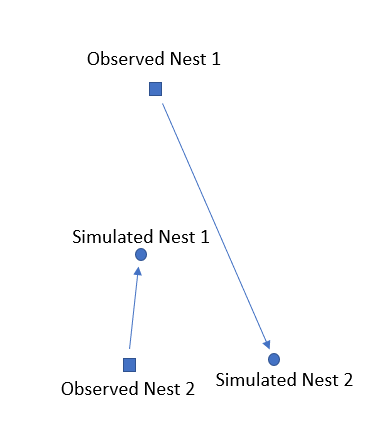
\includegraphics[width=0.3\linewidth]{subs1.PNG}}
 \subfloat[B]{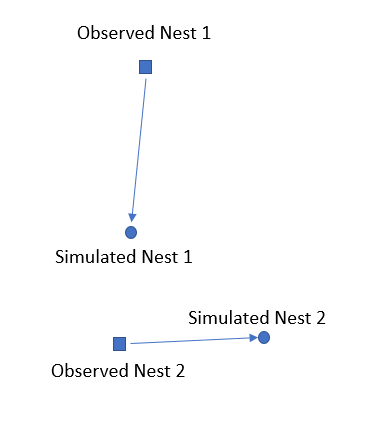
\includegraphics[width=0.3\linewidth]{subs2.PNG}}
\caption{[A] shows the shortest distance substitution in the deterministic scenario. [B] shows the more likely substitution that would be discarded in the deterministic scenario.}
\label{fig:1}
\end{figure*}

A better strategy would be the following. Assume that each particle that has been simulated up to time $T_i$ can be corrected in a finite number of ways when we receive a new set of observations $\vec{z}^{T_i}$. We also make the assumption that a nests can be only corrected once and if corrected at time $T_j$ it will not be corrected again in future times. These corrections are made with probability $H_{z^{T_i}}((\vec{A}^{T_i})' | \vec{A}^{T_i})_{\zeta}$, where $(\vec{A}^{T_i})'$ is the vector of the corrected nests at time $T_i$.

The probability $H_{z^{\tau_i}}((\vec{A}^{T_i})' | \vec{A}^{T_i})_{\zeta}$ of the new configuration of nests $\zeta$ will depend on the distances between the simulated nests and the observed nests in the following way. Let us consider a simulated nest $a_j$ and an observation $z_h$. Then $a_j$ can be corrected by $z_h$ with probability $p_{a_j z_h} = p(a_j \leftrightarrow z_h) = e^{-d_{a_j z_h}}$ where $d_{a_j z_h}$ is the Euclidean distance between $a_j$ and $z_h$. Notice that when the distance is $d_{s_j z_h} = 0$ the probability $p_{s_j z_h}$ is 1 and the observation coincide with the simulated nest. The probability of a certain new configuration of nests will therefore be $H_{z^{T_i}}((\vec{A}^{T_i})' | \vec{A}^{T_i})_{\zeta} \propto (\prod_{h = 1}^{M^{T_i}} (p_{a_j z_h}))_{\zeta}$ and after normalization $H_{z^{T_i}}((\vec{A}^{T_i})' | \vec{A}^{T_i})_{\zeta} = (\prod_{h = 1}^{M^{T_i}} (p_{a_j z_h}))_{\zeta} / \sum_{\zeta} (\prod_{h = 1}^{M^{T_i}} (p_{a_j z_h}))_{\zeta} $ where the sum is over all the possible configurations. Each set of simulated particles that have not been corrected, can be corrected in only a finite number of ways to produce an element of the non-empty finite set $O_{\vec{z}^{T_i}} (\vec{A}^{T_i})$ that contains all the allowed corrections. The correction is made selecting an element $(\vec{A}^{T_i})'$ from the set $O_{\vec{z}^{T_i}} (\vec{A}^T)$ with probability $H_{z^{T_i}}((\vec{A}^{T_i})' | \vec{A}^{T_i})_{\zeta}$. Configurations of nests where the distances between observed and simulated nests are small will be more probable than the one where those distances are big.

Let us call $s$ the number of simulated nests that we want to correct and $o$ the number of observed nests. The way we make the substitution is valid regardless of the values of $s$ and $o$ and the number of possible configuration is that obtained in ordered sampling without replacement. If we have more observed nests than simulated nests, we will correct all simulated nests and add all the remaining observed nests to the new configuration. Similarly if we have more simulated nests than observed one we will correct only the number of nests that we observe and leave the remaining nests to be corrected at a later stage.
It follows that the number of possible configurations will be $\frac{s!}{(s-o)!}$ if $s > o$, $o!$ if $s = o$, and $\frac{o!}{(o-s)!}$ if $o < s$.

Each time a nest is corrected its new location will correspond to the location of one of the observed nest and the time of observation will be corrected too with the observed one.

(NOTE: This might be an expensive step if we have a large number of nests. Should we consider a threshold (for example a maximum distance) over which the substitution cannot happen?) 
}

{\color{red}
\subsection{The calculation of the Weights} \label{subsec:weight}

At each iteration, in order to simulate via a two-step process in which we generate a sample and then correct in light of data, we propose to use an auxiliary variable in the following manner. The auxiliary variable will be the yet to be corrected sample $\vec{A}^{T_i}$, which is an element of the space $\Omega_{T_i}$. We will use a projection map $\pi$ to relate the augmented space $\Omega^*_{T_i} = \Omega_{T_i} \times \Omega'_{T_i}$ containing elements of the form $(\vec{A}^{T_i}, (\vec{A}')^{T_i})$ to the corrected state space $\Omega'_{T_i}$ containing elements of the form  $(\vec{A}')^{T_i}$. With the corrections defined in chapter \ref{subsec:corrections} the augmented space is $\Omega^*_{T_i} = \{ (\vec{A}^{T_i}, (\vec{A}')^{T_i}) : \vec{A}^{T_i} \in \Omega_{T_i} \, , \, (\vec{A}')^{T_i} \in O_{\vec{z}^{T_i}} (\vec{A}^{T_i}) \}$ Our strategy is to define a probability measure $\mathbb{P}^*$ having density $p^*$ on $\Omega^*_{T_i}$ such that the marginal density of $\mathbb{P}^*$ on $\Omega'$ is $\mathbb{P}$, that is $\mathbb{P} = \mathbb{P}^* \circ \pi^{-1}$, where $\mathbb{P}$ is the measure with density $p$ on $\Omega'_{T_i}$.

By the disintegration theorem there exists a family of measure $\{ \nu_{(\vec{A}')^{T_i}}\}_{(\vec{A}')^{T_i} \in \Omega'_{T_i}}$ on $\Omega^*_{T_i}$ such that for every measurable Borel function $ m : \Omega^*_{T_i} \rightarrow [0, \infty]$

\begin{equation*}
    \int_{\Omega^*_{T_i}} m((\vec{A}')^{T_i}, \vec{A}^{T_i}) \D \mathbb{P}^* = \int_{\Omega'_{T_i}} \Bigg( \int_{\pi^{-1}((\vec{A}')^{T_i})} m((\vec{A}')^{T_i}, \vec{A}^{T_i}) \D \nu_{(\vec{A}')^{T_i}}  \Bigg) \D \mathbb{P}((\vec{A}')^{T_i}).
\end{equation*}
It follows that for any event $B$,

\begin{align*}
    \mathbb{P}(B) = \mathbb{P}^*(\pi^{-1}(B)) &= \int_{\Omega^*_{T_i}} I_B (\pi((\vec{A}')^{T_i}, \vec{A}^{T_i})) p^* ((\vec{A}')^{T_i}, \vec{A}^{T_i} | \vec{Z}^{T_i}) \D \mathbb{P}^* \\ 
    &= \int_{\Omega'_{T_i}} I_B ((\vec{A}')^{T_i}) \Bigg[ \int_{\pi^{-1}((\vec{A}')^{T_i})} p^* ((\vec{A}')^{T_i}, \vec{A}^{T_i} | \vec{Z}^{T_i}) \D \nu_{(\vec{A}')^{T_i}} (\vec{A}^{T_i}) \Bigg] \D \mathcbb{P} (\vec{A}')^{T_i}.
\end{align*}
and hence

\begin{equation*}
    p((\vec{A}')^{T_i} | \vec{Z}^{T_i}) = \int_{\pi^{-1}((\vec{A}')^{T_i})} p^*((\vec{A}')^{T_i}, \vec{\vec{A}}^{T_i} | \vec{Z}^{T_i})\D \nu_{(\vec{A')}^{T_i}} (\vec{A}^{T_i}).
\end{equation*}
Moreover,

\begin{align*}
    E_{p}[l(\vec{(A')}^{T_i})]  &= \int_{\Omega'} l(\vec{(A')}^{T_i})\; p(\vec{(A')}^{T_i} | \vec{Z}^{T_i}) \D \mathbb{P}(\vec{(A')}^{T_i}) \\
    &= \int_{\Omega'} l(\vec{(A')}^{T_i})\Bigg[\int_{\pi^{-1}((\vec{A}')^{T_i})} p^*(\vec{(A')}^{T_i}, \vec{A}^{T_i} | \vec{Z}^{T_i}) \D \nu_{(\vec{A}')^{T_i}}(\vec{A}')^{T_i} \Bigg] \D \mathbb{P}{(\vec{A}')}^{T_i} \\ 
    &= \int_{\Omega^*} l(\pi(\vec{(A')}^{T_i}, \vec{A}^{T_i}))\; p^*(\vec{(A')}^{T_i}, \vec{A}^{T_i} | \vec{Z}^{T_i}) \D \mathbb{P}^*((\vec{A}')^{T_i}, \vec{A}^{T_i}) \\ 
    &= E_{p^*}[l(\pi (\vec{(A')}^{T_i}, \vec{A}^{T_i}))].
\end{align*}

Similarly, we define a density $\mathbb{Q}^*$ on $\Omega^*_{T_i}$ having probability function $q^*$ such that the marginal density of $\mathbb{Q}^*$ on $\Omega_{T_i}$ is $\mathbb{Q}$. We then use a sequential importance sampling approach to re-weight a sample of particle used for Monte Carlo estimation with respect to $q^*$, so that they can be used for Monte Carlo estimation with respect to $p^*$.

With the corrections introduced in chapter \ref{subsec:corrections} and reintroducing the particle subscript $k$ the joint density at $((\vec{A}_k')^{T_i}, \vec{A}_k^{T_i})$ sampled from the prior is

\begin{equation*}
    q^*(\vec{(A')}^{T_i}_k, \vec{A}^{T_i}_k | \vec{Z}^{T_{i-1}}) = q(\vec{A}^{T_i}_k | \vec{Z}^{T_{i-1}}) H_{z^{T_i}} (\vec{(A')}^{T_i}_k | \vec{A}^{{T_i}}_k).
\end{equation*}
and the density $p^*(\vec{(A')}^{T_i}_k, \vec{A}^{T_i}_k | \vec{Z}^{T_i})$ will be

\begin{equation*}
    p^*(\vec{(A')}^{T_i}_k, \vec{A}^{T_i}_k | \vec{Z}^{T}) = p(\vec{(A')}^{T_i}_k | \vec{Z}^{T_i}) u(\vec{(A)}^{T_i}) H_{(z')^{T_i}} (\vec{A}^{T_i}_k | \vec{(A')}^{{T_i}}_k)
\end{equation*}
where we choose $u$ to be the uniform density on $F((\vec{A}')^{T_i}, \vec{Z}^{T_i}) = \{ \vec{A}^{T_i} \in \Omega^{T_i} : (\vec{A}')^{T_i} = ?\}$ (NOTE: I need to fix this) and $H_{(z')^{T_i}} (\vec{A}^{T_i}_k | \vec{(A')}^{{T_i}}_k)$ represents a correction we would have made had we initially generated a sample $H_{(z')^{T_i}} (\vec{A}^{T_i}_k | \vec{(A')}^{{T_i}}_k)$.

(NOTE: here we will need to prove that p* is a proper density, that p* has marginal density p and the validity of the essential supports).
The weights will therefore be 

Applying importance sampling on the probability space $\Omega^*$ we have

\begin{align*}
    E_{p^*}[l(\pi (\vec{(A')}^{T_i}, \vec{A}^{T_i})] = \int_{\Omega^*} l(\pi((\vec{A}')^{T_i}, \vec{A}^{t})) \frac{p^*(\vec{(A')}^{T_i}, \vec{A}^{T_i}|\vec{Z}^{T_i})} {q^*(\vec{(A')}^{T_i}, \vec{A}^{T_i} | \vec{Z}^{T_{i-1}})} \\
    p(\vec{(A')}^{T_i}, \vec{A}^{T_i} | \vec{Z}^{T_{i-1}}) \; \D \vec{A}^{T_i} \approx \sum_{i=1}^n  w^{T_i}_i l(\pi (\vec{(A')}^{T_i}_i, \vec{A}^{T}_i))
\end{align*}
where the weights are given by

\begin{equation*}
    w^{T_i}_k \propto \frac{p^*(\vec{(A')}^{T_i}_k, \vec{A}^{T_i}_k | \vec{Z}^{T_i})} {q^*(\vec{(A')}^{T_i}_k, \vec{A}^{T_i}_k | \vec{Z}^{T_{i-1}})}
\end{equation*}
and therefore

\begin{equation*}
    w^{T_i}_k \propto \frac{q(\vec{(A')}^{T_i}_k | \vec{Z}^{T_{i-1}}) u(\vec{(A)}^{T_i}) H_{(z')^{T_i}} (\vec{A}^{T_i}_k | \vec{(A')}^{T_i}_k)}{p(\vec{A}^{T_i}_k | \vec{Z}^{T_{i-1}}) H_{z^{T_i}} (\vec{(A')}^{T_i}_k | \vec{A}^{T_i}_k)}
\end{equation*}
we notice now that the quantities $H_{(z')^{T_i}} (\vec{A}^{T_i}_k | \vec{(A')}^{T_T}_k)$ and $H_{z^{T_i}} (\vec{(A')}^{T_i}_k | \vec{A}^{T_i}_k)$ are identical at each step and will cancel out. Also $u$ and $r$ will cancel out after normalisation leaving

\begin{equation*}
    w^{T_i}_k = \frac{q(\vec{(A')}^{T_i}_k | \vec{Z}^{T_{i-1}})}{q(\vec{A}^{T_i}_k | \vec{Z}^{T_{i-1}})} \Bigg( \sum_{s=1}^n \frac{q(\vec{A}^{T_i}_s | \vec{Z}^{T_{i-1}})}{q(\vec{(A')}^{T_i}_s | \vec{Z}^{T_{i-1}})} \Bigg)
\end{equation*}


}


